\section{Užívateľské rozhranie}
\label{sec:Practice-UI}

Aplikácia sa zameriava na širokú škálu užívateľov - od náročného fotografa až po technicky neskúsenú
osobu, snažiacu sa vytvoriť čo najdôveryhodnejší záber scény. Preto by mala aplikácia minimalistickým 
a intuitívnym spôsobom ponúkať všetky potrebné nástroje a~možnosti, ktoré môže užívateľ využiť.

\begin{figure}[h!]
  \centering
  \begin{subfigure}{0.3\textwidth}
      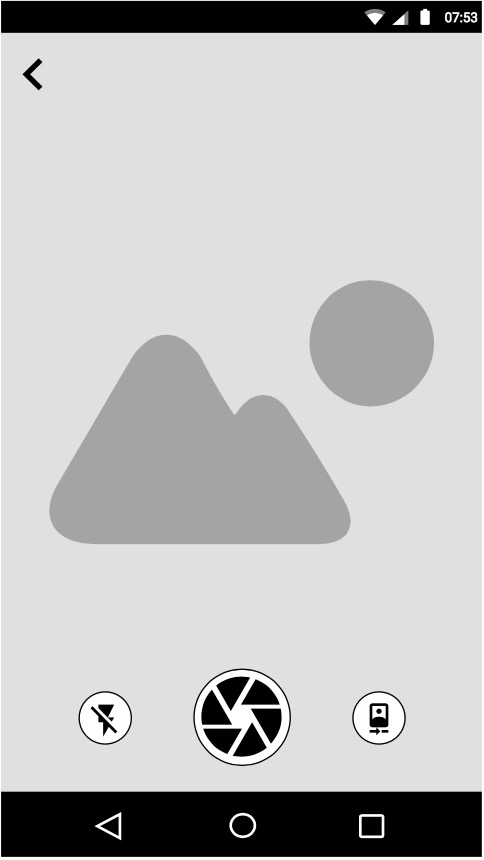
\includegraphics[width=\textwidth]{figures/ui/sketches/sketch-capture}
      \caption{Snímanie fotografie}
      \label{fig:sketch_capture}
  \end{subfigure}
  ~
  \begin{subfigure}{0.3\textwidth}
      
\includegraphics[width=\textwidth]{figures/ui/sketches/sketch-home}
      \caption{Domovská obrazovka}
      \label{fig:sketch_home}
  \end{subfigure}
  ~
  \begin{subfigure}{0.3\textwidth}
      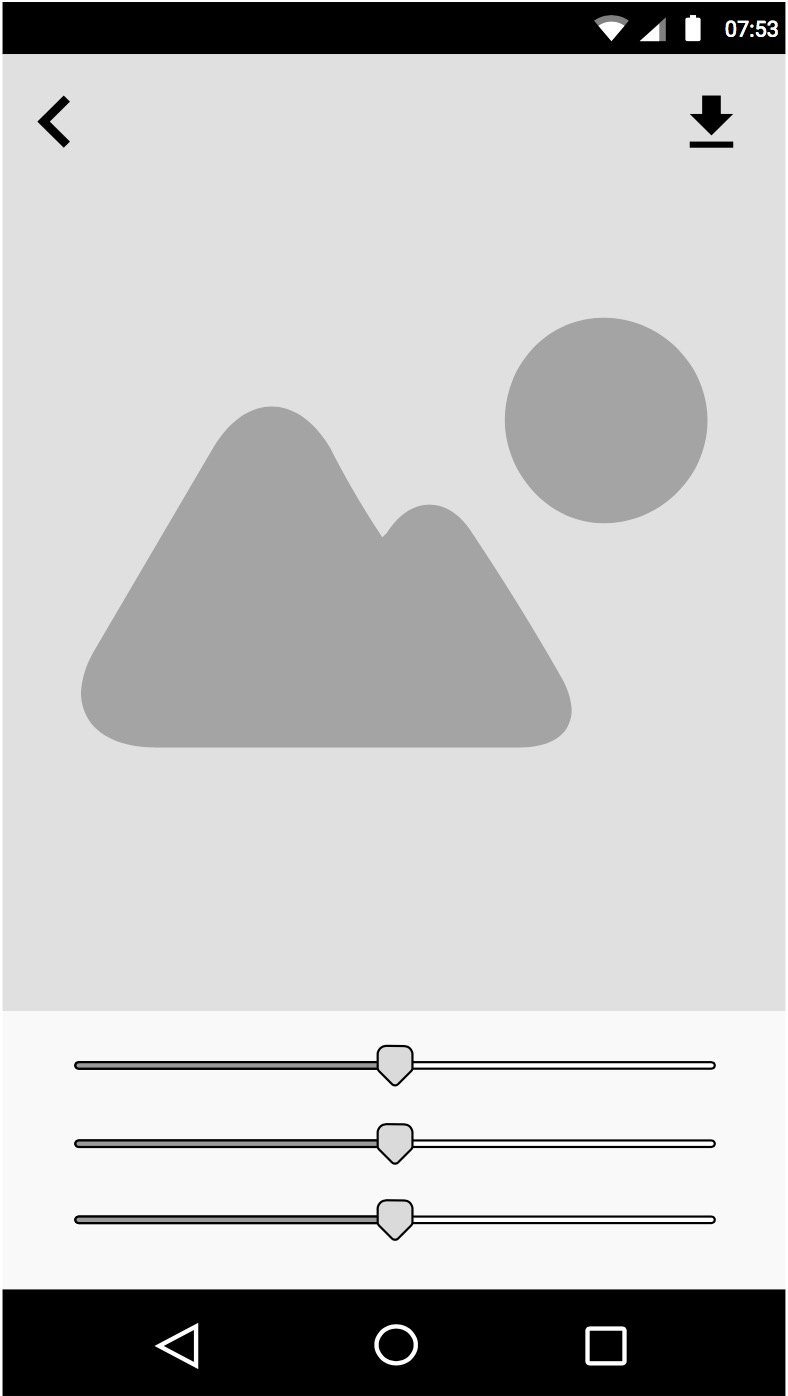
\includegraphics[width=\textwidth]{figures/ui/sketches/sketch-edit}
      \caption{Úprava fotografie}
      \label{fig:sketch_edit}
  \end{subfigure}
  \caption{Návrh obrazoviek užívateľského rozhrania}
  \label{fig:sketch_screens}
\end{figure}

Obrazovka \ref{fig:sketch_home} je príkladom toho, že užívateľ môže mať všetko čo potrebuje,
bez zbytočného zdĺhavého hľadania. Na vytvorenie HDR fotografie potrebujeme buď zachytiť aktuálnu scénu
fotoaparátom, alebo načítať súbor s HDR obsahom.

Po zachytení scény na fotografiu (obr. \ref{fig:sketch_capture}) alebo načítaní HDR obsahu a po spracovaní 
tohoto obsahu, má užívateľ na výber z rôznych techník mapovania tónov. Po výbere jednej z nich je
užívateľovi poskytnutá možnosť upravovania fotografie (obr. \ref{fig:sketch_edit}) do výslednej podoby 
pomocou prehľadnej ponuky nástrojov. Jednotlivé parametre sú spočiatku nastavené na vhodné východzie 
hodnoty, ktoré je možné po úpravach zresetovať. Na záver je možné výsledok uložiť do galérie. Rozhranie 
musí ponúkať aj možnosť vrátiť sa o obrazovku späť, na čo aplikácie z prieskumu existujúcich riešení 
často zabúdajú.

Náhľadová ikona (obr. \ref{fig:appIcon}) je navrhnutá, aby zachytila hlavnú myšlienku aplikácie.
Tri vrstvy s rozdielnými odtieňmi od najtmavšieho po najsvetlejší predstavujú fotografie zachytené
s rôznym časom expozície. Ich prelínanie naznačuje, že sa tieto snímky spájajú do jednej HDR fotografie.
Pôvodný čierno-biely návrh ikony časom nahradila varianta v~primárnych farbách užívateľského rozhrania.

\begin{figure}[h!]
    \centering
    
\includegraphics[width=0.3\textwidth]{figures/ui/logo/logo_bw}
    
\includegraphics[width=0.3\textwidth]{figures/ui/logo/logo}
    \caption{Ikona aplikácie}
    \label{fig:appIcon}
\end{figure}

Z domovskej obrazovky (obr. \ref{fig:homeScreen_hints}) je priamy prístup k nastaveniam aplikácie (obr.
\ref{fig:homeScreen_settings}). Nastavenia obsahujú možnosti definovania počtu vytvorených fotografií
v jednej sérii a zvolenie kroku pre algoritmus vyberajúci vhodné časy expozície (podkapitola
\ref{sec:Practice-ExpoSelector}).

\begin{figure}[h!]
    \centering
    \begin{subfigure}{0.35\textwidth}
        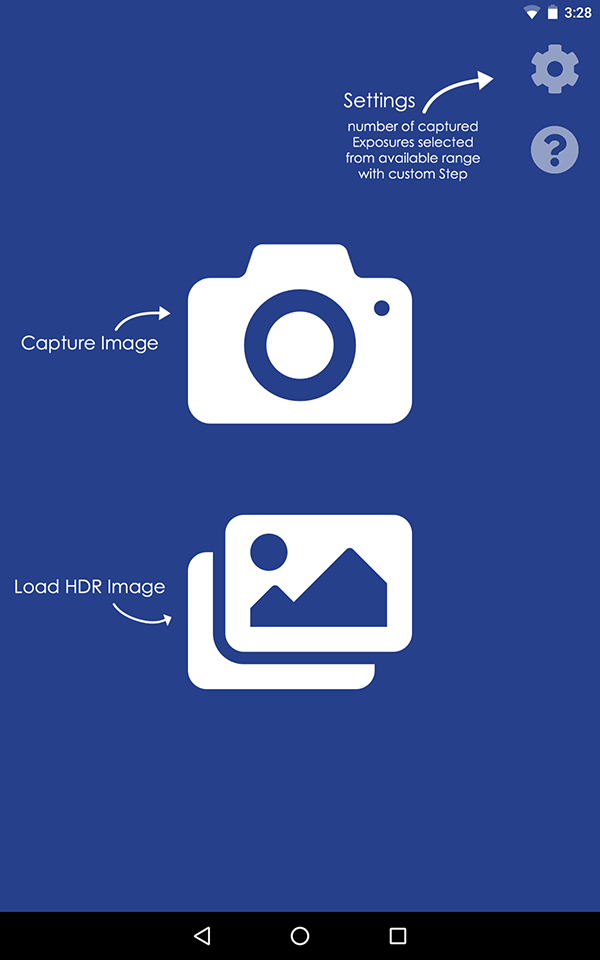
\includegraphics[width=\textwidth]{figures/ui/home/screenHome}
        \caption{Popis obrazovky}
        \label{fig:homeScreen_hints}
    \end{subfigure}
    ~
    \begin{subfigure}{0.35\textwidth}
        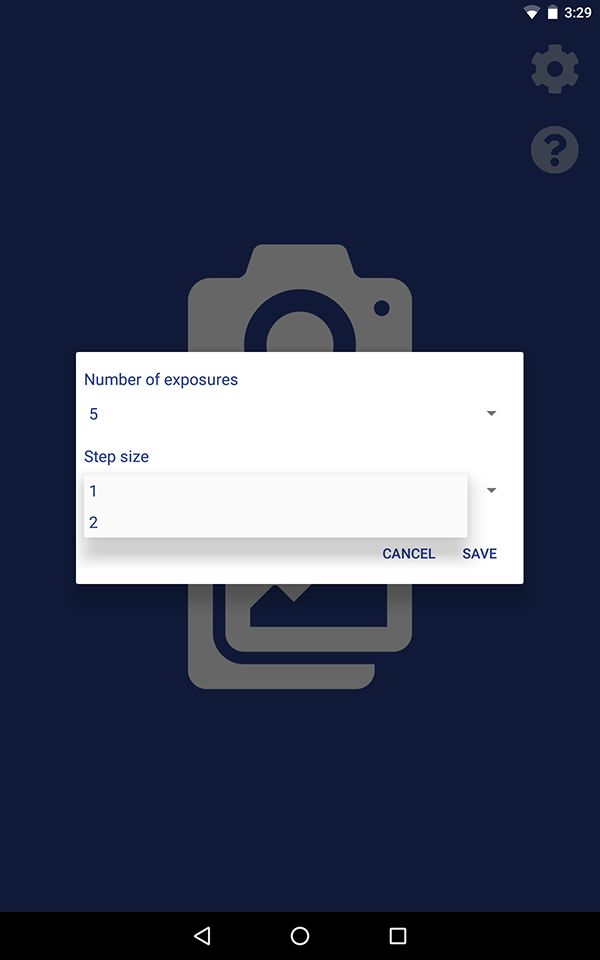
\includegraphics[width=\textwidth]{figures/ui/home/dialogSettings}
        \caption{Nastavenia aplikácie}
        \label{fig:homeScreen_settings}
    \end{subfigure}
    \caption{Domovská obrazovka}
    \label{fig:homeScreen}
\end{figure}

\subsection*{Android Fragment}

\begin{figure}[h!]
    \centering
    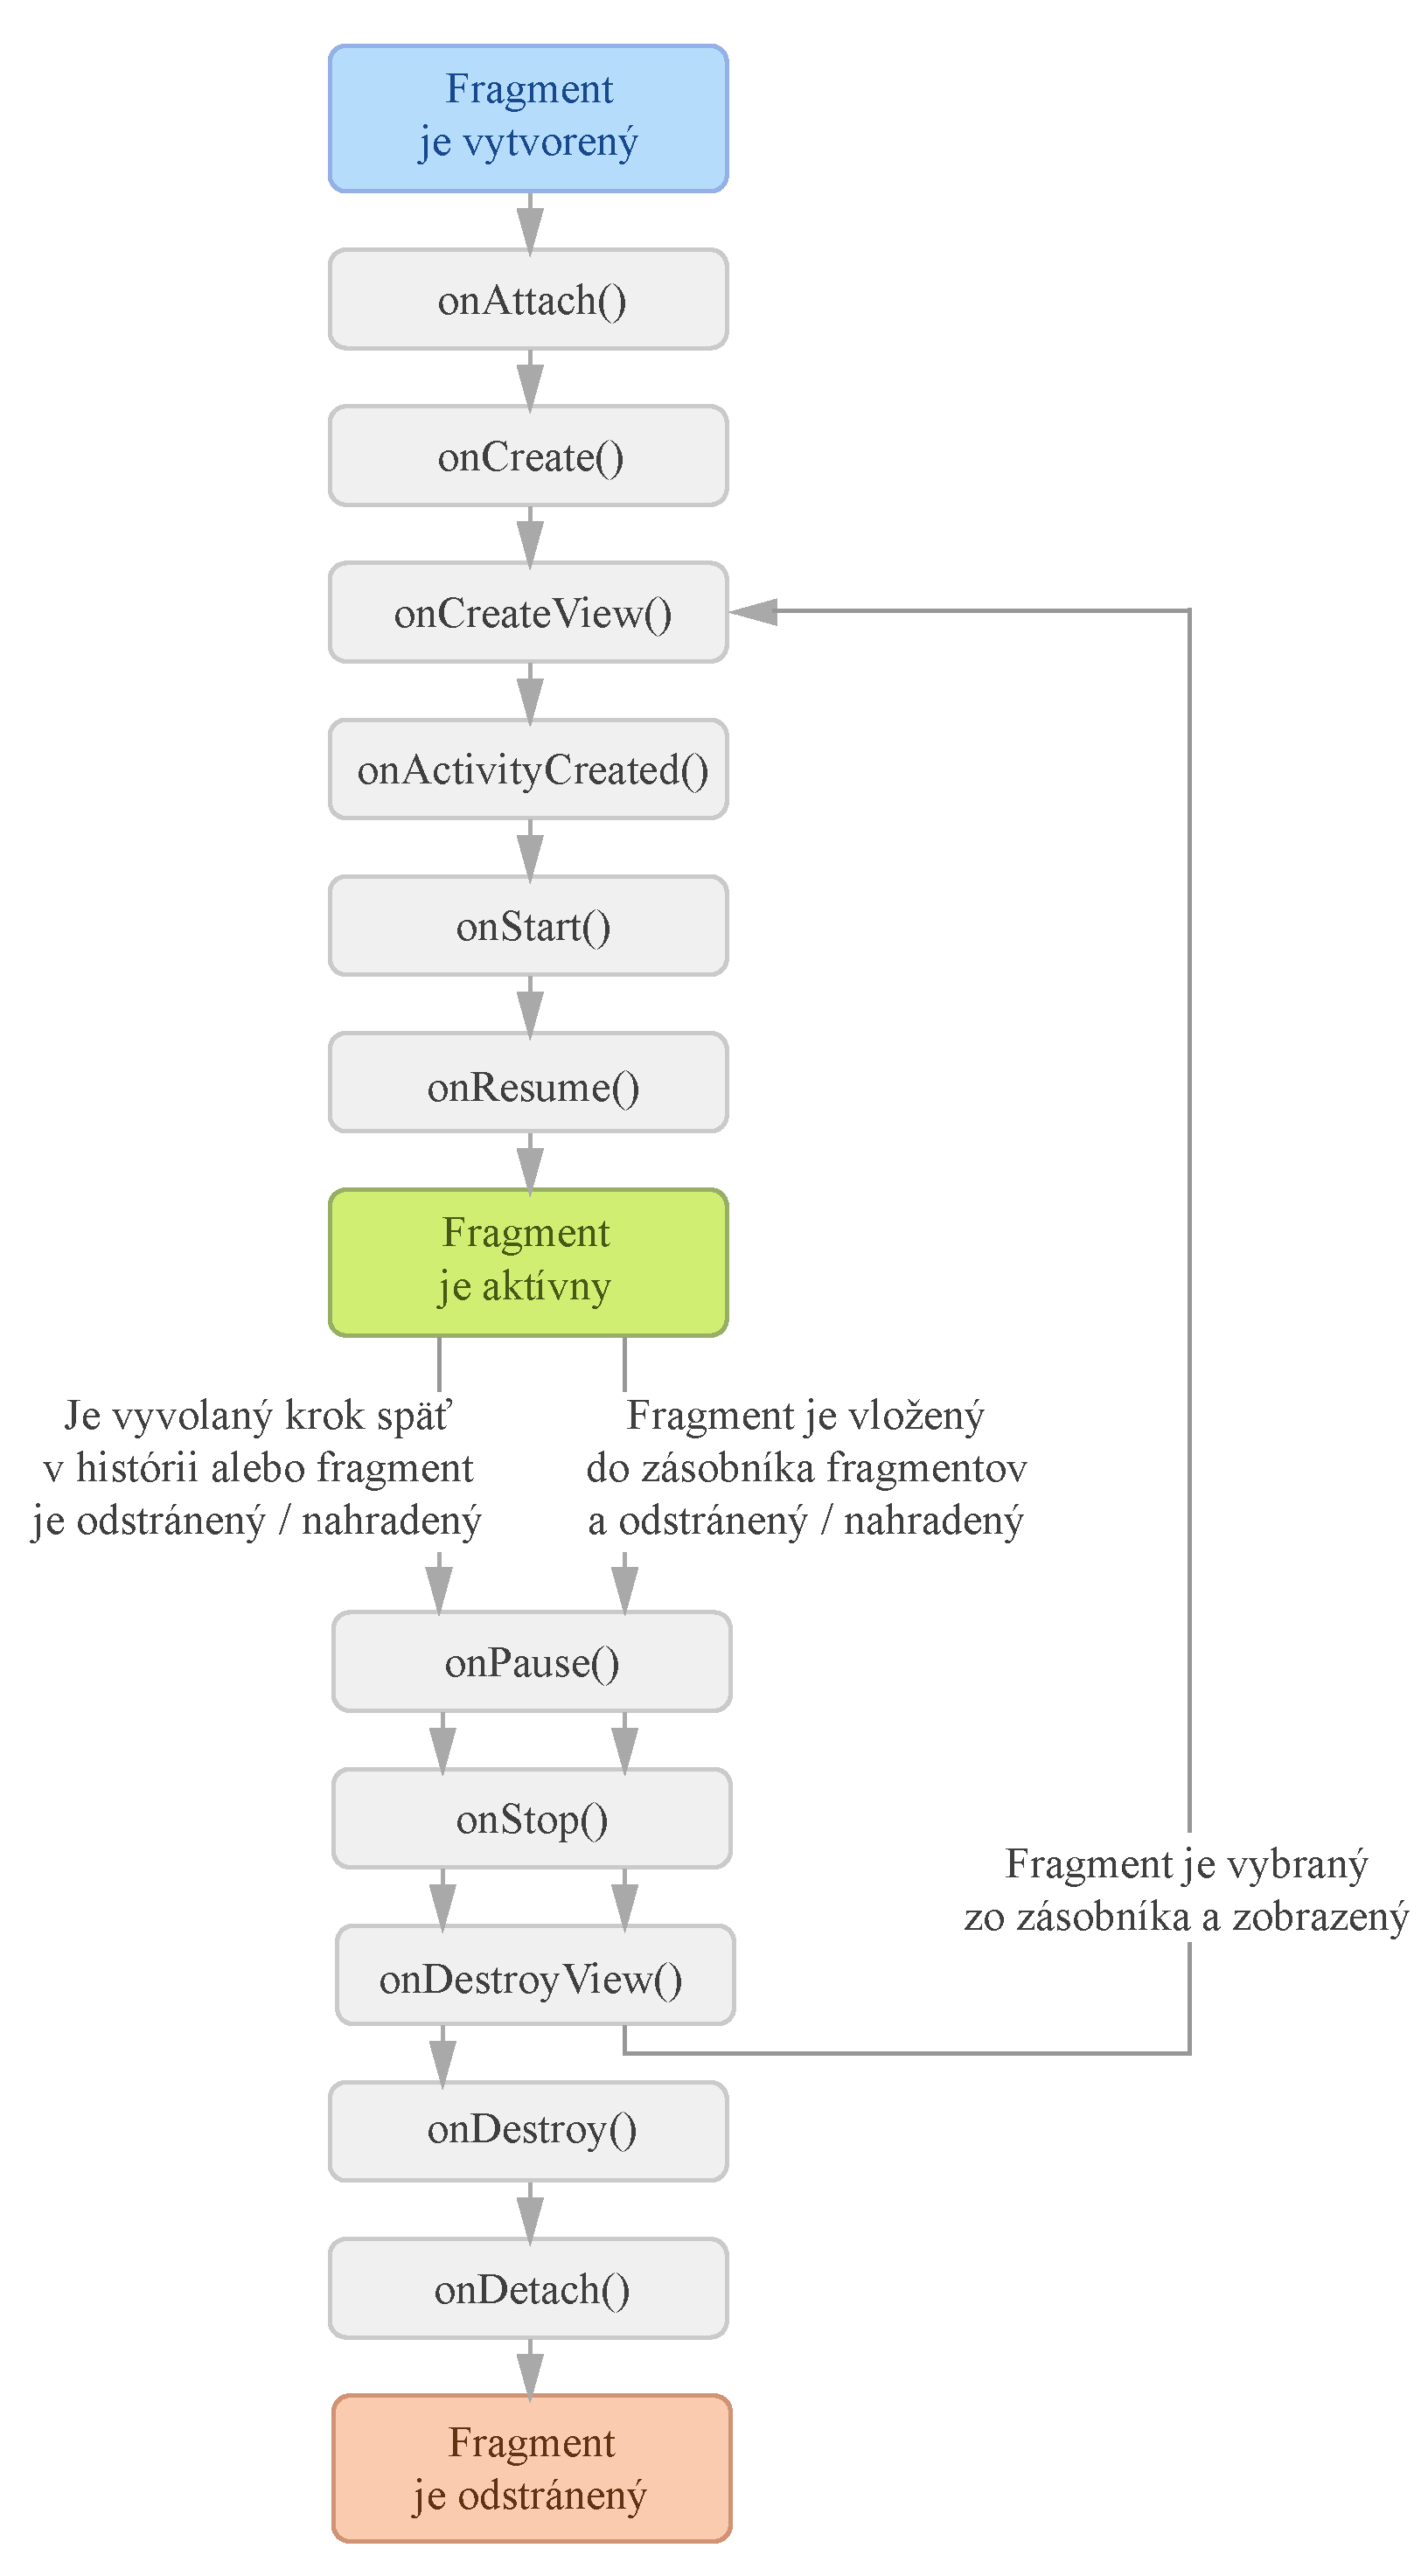
\includegraphics[width=0.5\textwidth]{figures/ui/fragment_lifecycle}
    \caption{Životný cyklus Fragmentu \cite{Android}}
    \label{fig:fragment_lifecycle}
\end{figure}

Jednotlivé obrazovky aplikácie sú vytvorené využitím Android Fragmentov. \texttt{Fragment} popisuje vymedzenú
časť užívateľského rozhrania, ktorú je možné vkladať, alebo odoberať počas behu aktivity. 
V hlavnej obrazovke aktivity je definovaný \texttt{FrameLayout} \texttt{container}, do ktorého sa podľa
situácie vkladajú obrazovky typu Fragment.

V triede \texttt{Main} aplikácie vkladáme jednotlivé obrazovky pomocou \texttt{FragmentTransaction} transakcií,
ku ktorým vytvára prístup \texttt{FragmentManager}.

\begin{lstlisting}[morekeywords={ExampleFragment,FragmentManager,FragmentTransaction,R}]
ExampleFragment newFragment = new ExampleFragment();

FragmentManager manager = getSupportFragmentManager();
FragmentTransaction transaction = manager.beginTransaction();

transaction.replace(R.id.fragment_container, newFragment);
transaction.addToBackStack(null);
transaction.commit();
\end{lstlisting}

Zásobník \texttt{BackStack} slúži na pohybovanie sa v histórii fragmentov aplikácie. To znamená, že ak užívateľ klikne
na tlačidlo späť, zo zásobníka sa vyberie posledný aktívny fragment a zobrazí sa. Typ našej aplikácie tento zásobník
nevyžaduje. Tlačidlá späť slúžia primárne na vrátenie sa na domovskú obrazovku, prípadne na obrazovku s výberom
operátora mapovania tónov.

Vykreslenie obrazovky v rozhraní zabezpečuje objekt \texttt{LayoutInflater}. Prvky a rozloženie obrazovky
je definované v jazyku XML.
\begin{lstlisting}[morekeywords={View, LayoutInflater, ViewGroup, Bundle}]
public View onCreateView(LayoutInflater inflater, ViewGroup container, Bundle savedInstanceState) {
    return inflater.inflate(R.layout.new_fragment, container, false)
}                                  
\end{lstlisting}
